\documentclass{standalone}
\usepackage{pgfplots}
\pgfplotsset{compat=1.18}

\usetikzlibrary{decorations.markings}
\usetikzlibrary{arrows.meta}


\begin{document}

% Electromagnetic wave - circular polarization - color
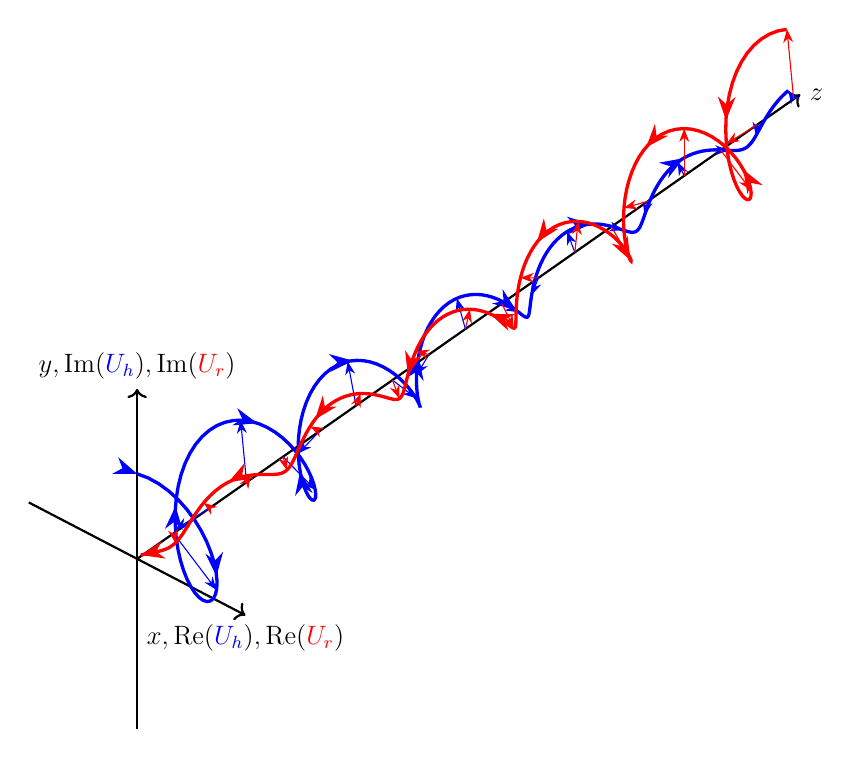
\begin{tikzpicture}[x=(35:0.9), y=(90:0.9), z=(-45:1.1),
axis/.style={black, thick,->},
vector/.style={>=Stealth,->},
scale=0.8, transform shape]

\large
\pgfmathsetmacro{\A}{1.5}
\pgfmathsetmacro{\om}{1.3}
\pgfmathsetmacro{\maxDomain}{1.5}
\pgfmathsetmacro{\nNodes}{6} % use even number
\pgfmathsetmacro{\nVectorsPerNode}{2}
\pgfmathsetmacro{\N}{\nNodes*40}
\pgfmathsetmacro{\decay}{0.15}
\pgfmathsetmacro{\xmax}{\nNodes*pi/2*1.01}
\pgfmathsetmacro{\nVectors}{\nVectorsPerNode*\nNodes*1.5}

% MAIN AXES
\draw[axis] (0,0,0) -- ++(\xmax*1.5,0,0) node[right] {$z$};
\draw[axis] (0,-\A*2.0,0) -- (0,\A*2.0,0) node[above] {$y, \mathrm{Im}({\color{blue}U_{h}}),
\mathrm{Im}({\color{red}U_{r}})$};
\draw[axis] (0,0,-\A*2.0) -- (0,0,\A*2.0) node[below] {$x, \mathrm{Re}({\color{blue}U_{h}}),
\mathrm{Re}({\color{red}U_{r}})$};


% blue spiral

\pgfmathdeclarefunction{fx}{2}{%
    % #1: z in radians
    % #2: argument
    \pgfmathparse{\A*exp(-#1*\decay)*cos(deg(\om*2.0*#1)+#2)}%
}

\pgfmathdeclarefunction{fy}{2}{%
    % #1: z in radians
    % #2: argument
    \pgfmathparse{\A*exp(-#1*\decay)*sin(deg(\om*2.0*#1)+#2)}%
}

\draw[very thick,variable=\t,domain=0:\nNodes*pi/2*\maxDomain,samples=\N,blue, postaction={decorate},
decoration={markings, mark=between positions 0 and 1 step 0.1 with {\arrow{Stealth}}}]
plot (\t,{fx(\t, 0)},{fy(\t, 0)});

% draw vectors
\foreach \k [evaluate={\t=\k*pi/2/\nVectorsPerNode; \angle=\k*90/\nVectorsPerNode;}] in {1,...,\nVectors}{
    \draw[vector,blue] (\t,0,0) -- ++(0,{fx(\t, 0)},{fy(\t, 0)});
}




% red spiral

\pgfmathdeclarefunction{fx2}{2}{%
    % #1: z in radians
    % #2: argument
    \pgfmathparse{\A*exp(-(pi*5-#1)*\decay)*cos(deg(\om*2.0*#1)+#2)}%
}

\pgfmathdeclarefunction{fy2}{2}{%
    % #1: z in radians
    % #2: argument
    \pgfmathparse{\A*exp(-(pi*5-#1)*\decay)*sin(deg(\om*2.0*#1)+#2)}%
}

\draw[very thick,variable=\t,domain=0:\nNodes*pi/2*\maxDomain,samples=\N,red, postaction={decorate},
decoration={markings, mark=between positions 0 and 1 step 0.1 with {\arrowreversed{Stealth}}}]
plot (\t,{fx2(\t, 180/4)},{fy2(\t, 180/4)});


% draw vectors
\foreach \k [evaluate={\t=\k*pi/2/\nVectorsPerNode; \angle=\k*90/\nVectorsPerNode;}] in {1,...,\nVectors}{
    \draw[vector,red] (\t,0,0) --
    ++(0,{fx2(\t, 180/4)},{fy2(\t, 180/4)});
}

\end{tikzpicture}


\end{document}
